% !TEX TS-program = pdflatex
% !TEX encoding = UTF-8 Unicode

\documentclass{beamer}

\usetheme{Boadilla}
\setbeamerfont{frametitle}{size=\small}

\usepackage[english,russian]{babel}
\usepackage[utf8]{inputenc}
\usepackage{times}

\newcommand{\docId}{Отчёт}
\newcommand{\theAuthor}{\textcopyright  АНО ``Образовательный квартал'' 2014}
\newcommand{\myaa}{-1}
\newcommand{\myab}{-1}
\newcommand{\myac}{-1}
\newcommand{\myad}{-1}
\newcommand{\socioSizeCommentA}{В связи с малым количеством сотрудников в Вашей организации (меньше 7~человек) социометрический анализ не представляется возможным.}
\newcommand{\socioSizeCommentB}{В связи с количеством сотрудников в Вашей организации (не более 11~человек) анализировались только 2 верхних выбора по указанным вопросам.}
\newcommand{\socioSizeCommentC}{В связи с количеством сотрудников в Вашей организации (не более 16~человек) анализировались только 3 верхних выбора по указанным вопросам.}
\newcommand{\socioSizeCommentD}{В связи с количеством сотрудников в Вашей организации (не более 21~человек) анализировались только 4 верхних выбора по указанным вопросам.}
\newcommand{\socioSizeCommentE}{\ }


\makeatother
\setbeamertemplate{footline}
{
  \leavevmode%
  \hbox{%
  \begin{beamercolorbox}[wd=.2\paperwidth,ht=2.25ex,dp=1ex,center]{doc number}%
    \usebeamerfont{}\docId\  \No\  T-\internalId
  \end{beamercolorbox}%
  \begin{beamercolorbox}[wd=.7\paperwidth,ht=2.25ex,dp=1ex,center]{doc comment}%
    \usebeamerfont{}\theAuthor\hspace*{3em}
  \end{beamercolorbox}%
  \begin{beamercolorbox}[wd=.1\paperwidth,ht=2.25ex,dp=1ex,center]{doc comment}%
    \insertframenumber{} \hspace*{1ex}
  \end{beamercolorbox}}%
  \vskip0pt%
}
\makeatletter
\setbeamertemplate{navigation symbols}{}


\usenavigationsymbolstemplate{}
\subtitle{Анализ педагогического состава учебного заведения 
на основе проведенного анкетирования}

\author{}
\institute{}
\date{}

\begin{document}

\title[МАОУ Заводопетровская СОШ] {Исследование социального капитала МАОУ Заводопетровская СОШ}

\subtitle{Анализ педагогического состава учебного заведения на основе проведенного анкетирования}

%=====================================================
\begin{frame}{1.	Состав группы анкетируемых}

\tiny


\begin{itemize}
\item Количество административных и педагогических работников – \nTotal.
\item Количество заполнивших анкету – \nParticipated.
\item Административные работники – \numBoss.
\item Педагогические работники – \numTeacher.
\item Пол \\
\begin{tabular}{|c|c|} \hline
мужчины &  женщины \\ \hline
\numMen     &   \numWomen   \\ \hline
\end{tabular}

\item Возраст \\
\noindent
\begin{tabular}{|c|c|c|c|} \hline
до 25 лет &  25 -- 35  лет &  36 -- 55 лет & свыше 55 лет \\ \hline
\numYoung     &   \numMidAge         &   \numSenior        & \numOld  \\ \hline
\end{tabular}

\item Образование

\begin{tabular}{|c|c|c|c|c|c|c|} \hline
Среднее  & Среднее  & Высшее    & Иное  & Послевузовское \\
специальное & специальное & педагогическое & высшее & (аспирантура,\\
(педагог.)       & (не педагог.)   & (спец., маг., бак.) & &  докторантура) \\ \hline
\numEduA & \numEduB & \numEduC, \numEduD, \numEduE & \numEduF & \numEduG \\ \hline
\end{tabular}

\item Педагогический стаж \\
\noindent
\begin{tabular}{|c|c|c|c|} \hline
 до 5 лет &  6 -- 10 лет &  11 -- 20 лет & больше 20 лет \\ \hline
 \numExpA    &  \numExpB    & \numExpC & \numExpD \\ \hline
\end{tabular}

\item Стаж работы в данном образовательном учреждении \\
\noindent
\begin{tabular}{|c|c|c|c|} \hline
 до 5 лет &  6 -- 10  лет &  11 -- 20 лет & больше 20 лет \\ \hline
 \numExpHereA & \numExpHereB & \numExpHereC & \numExpHereD \\ \hline
\end{tabular}

\item Квалификационная категория \\
\noindent
\begin{tabular}{|c|c|c|c|c|} \hline
 Не проходил &  Аттестован & 2-я &  1-я  & Высшая \\ 
 аттестацию   &  на соотв. & категория &  категория  & категория \\ \hline
 \numTechCatA & \numTechCatB & \numTechCatC &  \numTechCatD &  \numTechCatE \\ \hline
\end{tabular}

\end{itemize}
\end{frame}



%=====================================================
\begin{frame}{1.1. Список сотрудников}
\begin{itemize}
\fontsize{3pt}{4}\selectfont
\input{nameslist.tex}
\end{itemize}
\end{frame}




%=====================================================
\begin{frame}{2. Уровень горизонтального доверия}

Вступление с определением понятия области исследования и отсылкой к подробностям в Методических рекомендациях.

\end{frame}




%=====================================================
\begin{frame}{2.1. Декларируемый уровень доверия к коллегам }

\tiny
В этом разделе обсуждаем декларируемое доверие, то есть то, насколько Ваши коллеги в целом (можно сказать, теоретически) признают важность доверия, сотрудничества и обмена опытом. Это не означает, что они руководствуются этими принципами в своем повседневном профессиональном поведении, но считают правильным декларировать именно такую жизненную позицию.
\bigskip

В данном разделе анализируются ответы на вопросы Б13, Б14, Б10, Б25, Б30:
\bigskip

\begin{itemize}

\item [Б13] Есть ли у Вас профессиональные задачи, решение которых требует знакомства с опытом работы других педагогов (преподавателей, воспитателей) Вашей образовательной организации?

\item [Б14] Считаете ли Вы полезным и правильным посещение педагогами (преподавателями, воспитателями)  занятий и мероприятий (не открытых, т.е. специально не подготовленных), проводимых другими?

\item [Б10] С Вашей точки зрения, большинству коллег в Вашей образовательной организации можно доверять (доверие - уверенность в том, что, если Вы сказали коллеге о своих проблемах или ошибках, то эта информация не будет использована Вам во вред)?

\item[Б25] Как Вам кажется, нравится ли педагогам (преподавателям, воспитателям) то, что Вы посещаете их занятия и мероприятия?

\item[Б30] Спокойно ли Вам коллеги предоставляют свой кабинет (группу), оборудование для проведения урока (занятия или мероприятия)?

\end{itemize}

\end{frame}



%=====================================================
\begin{frame}{2.1.1. Признание ценности сотрудничества и доверия (сводный результат) }


\tiny

На диаграмме представлен сводный результат по вопросам Б13, Б14.
\bigskip

Б13. Есть ли у Вас профессиональные задачи, решение которых требует знакомства с опытом работы других педагогов (преподавателей, воспитателей) Вашей образовательной организации?
\smallskip

Б14. Считаете ли Вы полезным и правильным посещение педагогами (преподавателями, воспитателями)  занятий и мероприятий (не открытых, т.е. специально не подготовленных), проводимых другими?
\bigskip

\begin{columns}
\begin{column}{0.4\textwidth} 
\centering
\includegraphics[width=4cm, height=4cm]{pie211.png}
\end{column}
\begin{column}{0.6\textwidth} \begin{tabular}{l} 
 Ответили утвердительно   \\ 
(``да'' или ``скорее да, чем нет'')  ---   \valBAAyesNumP\% \\ [0.3cm]
 Ответили отрицательно  \\ 
 (``нет'' или ``скорее нет, чем да'') ---  \valBAAnoNumP\% \\ 
\end{tabular}
\end{column}
\end{columns}

\end{frame}



%=====================================================
\begin{frame}{2.1.2. Признание ценности сотрудничества и доверия (группы по возрасту) }

\tiny

На диаграмме представлен результат по вопросам Б13, Б14 с разбивкой по возрасту:
\bigskip

\centering 

\begin{tabular}{|l|c|c|c|c|} \hline
& до 25 лет &  25 -- 35  лет &  36 -- 55 лет & свыше 55 лет \\ \hline
Ответили утвердительно & & & & \\
(``да'' или ``скорее да, чем нет'')  & \valBAByesNumA     & \valBAByesNumB    &   \valBAByesNumC    & \valBAByesNumD  \\ \hline
Ответили отрицательно  & & & & \\
(``нет'' или ``скорее нет, чем да'') & \valBABnoNumA     &  \valBABnoNumB    &   \valBABnoNumC     & \valBABnoNumD  \\ \hline
\end{tabular}
\bigskip

\begin{tabular}{cccc}
\includegraphics[width=2.2cm, height=2.2cm]{pie212a.png} & 
\includegraphics[width=2.2cm, height=2.2cm]{pie212b.png} & 
\includegraphics[width=2.2cm, height=2.2cm]{pie212c.png} & 
\includegraphics[width=2.2cm, height=2.2cm]{pie212d.png} \\
до 25 лет &  25 -- 35  лет &  36 -- 55 лет & свыше 55 лет \\
\end{tabular}

\end{frame}



%=====================================================
\begin{frame}{2.1.3. Признание ценности сотрудничества и доверия (группы по квалификационной категории) }

\tiny

На диаграммах представлен результат по вопросам Б13, Б14 с разбивкой по квалификационной категории.
\bigskip

\centering 

\begin{tabular}{|l|c|c|c|c|c|} \hline
  & Не проходил &  Аттестован & 2-я &  1-я  & Высшая \\ 
 &  аттестацию   &  на соотв. & категория &  категория  & категория \\ \hline
Ответили  & & & & & \\
утвердительно  & \valBACyesNumA  &  \valBACyesNumB  & \valBACyesNumC  & \valBACyesNumD  & \valBACyesNumE \\ 
(Да, cкорее да...) & & & & & \\ \hline
Ответили   & & & & & \\
отрицательно & \valBACnoNumA   & \valBACnoNumB  & \valBACnoNumC  & 
\valBACnoNumD & \valBACnoNumE \\ 
(Нет, cкорее нет...) & & & & & \\ \hline
\end{tabular}

\bigskip

\begin{tabular}{ccccc}
\includegraphics[width=2cm, height=2cm]{pie213a.png} & 
\includegraphics[width=2cm, height=2cm]{pie213b.png} & 
\includegraphics[width=2cm, height=2cm]{pie213c.png} & 
\includegraphics[width=2cm, height=2cm]{pie213d.png} & 
\includegraphics[width=2cm, height=2cm]{pie213e.png} \\
 Не проходили &  Аттестованы & 2-я &  1-я  & Высшая \\ 
  аттестацию   &  на соотв. & категория &  категория  & категория \\ 
\end{tabular}

\end{frame}



%=====================================================
\begin{frame}{2.1.4. Данные по вопросам, включенным в блок ``Декларируемый уровень доверия к коллегам'' }

\tiny


\begin{tabular}{lccl}

 & Да & Нет &\\

\begin{minipage}{0.62\textwidth}
Б10. ``С Вашей точки зрения, большинству коллег в Вашей образовательной организации можно доверять (доверие - уверенность в том, что, если Вы сказали коллеге о своих проблемах или ошибках, то эта информация не будет использована Вам во вред)?''
\end{minipage}
& \valBADyesNumA & \valBADnoNumA &
\begin{minipage}{1.55cm}
\includegraphics[width=1.5cm, height=1.5cm]{pie214a.png}
\end{minipage}
\\[0.5cm]

\begin{minipage}{0.62\textwidth}
Б13.  ``Есть ли у Вас профессиональные задачи, решение которых требует знакомства с опытом работы других педагогов (преподавателей, воспитателей) Вашей образовательной организации?''
\end{minipage}
& \valBADyesNumB & \valBADnoNumB &
\begin{minipage}{1.55cm}
\includegraphics[width=1.5cm, height=1.5cm]{pie214b.png}
\end{minipage}
\\[0.5cm]

\begin{minipage}{0.62\textwidth}
Б14. ``Считаете ли Вы полезным и правильным посещение педагогами (преподавателями, воспитателями)  занятий и мероприятий (не открытых, т.е. специально не подготовленных), проводимых другими?''
\end{minipage}
& \valBADyesNumC & \valBADnoNumC &
\begin{minipage}{1.55cm}
\includegraphics[width=1.5cm, height=1.5cm]{pie214c.png}
\end{minipage}
\\[0.5cm]

\begin{minipage}{0.62\textwidth}
Б25. ``Как Вам кажется, нравится ли педагогам (преподавателям, воспитателям) то, что Вы посещаете их занятия и мероприятия?''
\end{minipage}
& \valBADyesNumD & \valBADnoNumD &
\begin{minipage}{1.55cm}
\includegraphics[width=1.5cm, height=1.5cm]{pie214d.png}
\end{minipage}
\\[0.5cm]

\begin{minipage}{0.62\textwidth}
Б30. ``Спокойно ли Вам коллеги предоставляют свой кабинет (группу), оборудование для проведения урока (занятия или мероприятия)?''
\end{minipage}
& \valBADyesNumE & \valBADnoNumE &
\begin{minipage}{1.55cm}
\includegraphics[width=1.5cm, height=1.5cm]{pie214e.png}
\end{minipage}

\end{tabular}

\end{frame}




%=====================================================
\begin{frame}{2.2. Регламентированный и нерегламентированный обмен опытом}

\tiny

В данном разделе анализируются ответы на вопросы Б3, Б4, Б21, Б22, Б24:
\bigskip

\begin{itemize}

\item [Б3] Посещение чужих открытых уроков. ``Как часто за последний учебный год Вы посещали открытые уроки (занятия, мероприятия) педагогов (преподавателей)  Вашей образовательной организации?''

\item [Б4] Проведение открытых уроков. ``Как часто за последний учебный год Вы давали открытые уроки (занятия, мероприятия)?''

\item [Б21] Частота посещения не подготовленных заранее занятий респондента коллегами-педагогами. ``Как часто коллеги-педагоги (преподаватели, воспитатели) за последний учебный год посещали Ваши занятия и мероприятия (не открытые, т.е. которые вы специально не готовили)?''

\item [Б22] Частота посещения респондентом заранее не подготовленных занятий и мероприятий коллег. ``Как часто за последний учебный год Вам приходилось бывать на занятиях и мероприятиях (не открытых, т.е. которые они специально не готовили) педагогов (преподавателей, воспитателей) Вашей образовательной организации?''

\item [Б24] Обычные действия после посещения открытых и неподготовленных занятий. ``После посещения занятий  и мероприятий (открытых и неоткрытых)  в нашей образовательной организации  обычно:''

\end{itemize}

\end{frame}



%=====================================================
\begin{frame}{2.2.1. Частотность обмена опыта в организации (сводный результат)}


\tiny

На диаграмме представлен сводный результат по вопросам Б3, Б4, Б21, Б22.
\bigskip

\begin{columns}
\begin{column}{0.4\textwidth} 
\centering
\includegraphics[width=4cm, height=4cm]{pie221.png}
\end{column}
\begin{column}{0.6\textwidth} \begin{tabular}{l} 
 Достаточно часто  \\ 
(``Раз в неделю'' или ``Раз в месяц'')  ---  \valBBAyesNumP\% \\ [0.3cm]
Достаточно редко  \\ 
 (``Раз в полугодие'' или ``Ещё реже'') ---  \valBBAnoNumP\% \\ 
\end{tabular}
\end{column}
\end{columns}
\bigskip

На диаграмме сводный результат по вопросам обмена опытом. Насколько часто, с Вашей точки зрения, сотрудники должны обмениваться опытом? Как соотносится Ваше представление с реальной ситуацией, обозначенной на диаграмме? 

\end{frame}

%=====================================================
\begin{frame}{2.2.2. Частотность обмена опыта в организации (группы по возрасту) }

\tiny

На диаграмме представлен результат по вопросам Б3, Б4, Б21, Б22 с разбивкой по возрасту:
\bigskip

\centering 

\begin{tabular}{|l|c|c|c|c|} \hline
& до 25 лет &  25 -- 35  лет &  36 -- 55 лет & свыше 55 лет \\ \hline
Ответили утвердительно & & & & \\
(``Раз в неделю'' или ``Раз в месяц'')  & \numYoung     &   \numMidAge         &   \numSenior        & \numOld  \\ \hline
Ответили отрицательно  & & & & \\
(``Раз в полугодие'' или ``Ещё реже'') & \numYoung     &   \numMidAge         &   \numSenior        & \numOld  \\ \hline
\end{tabular}
\bigskip

\begin{tabular}{cccc}
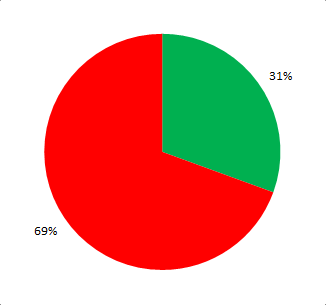
\includegraphics[width=2.2cm, height=2.2cm]{diag.png} & 
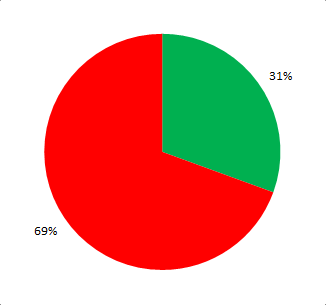
\includegraphics[width=2.2cm, height=2.2cm]{diag.png} & 
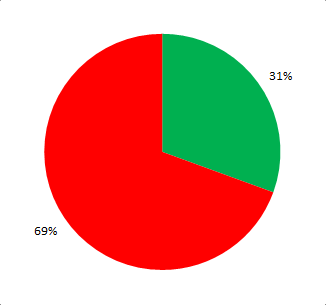
\includegraphics[width=2.2cm, height=2.2cm]{diag.png} & 
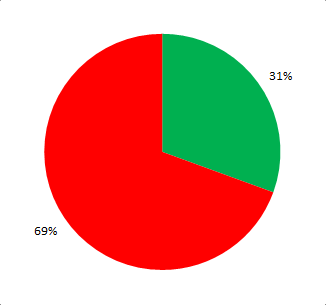
\includegraphics[width=2.2cm, height=2.2cm]{diag.png} \\
до 25 лет &  25 -- 35  лет &  36 -- 55 лет & свыше 55 лет \\
\end{tabular}

\end{frame}



%=====================================================



%=====================================================
\begin{frame}{2.2.4. Данные по вопросам, включенным в блок ``Регламентированный и нерегламентированный обмен опытом'' }

\tiny

\begin{tabular}{lccl}

 & Раз в месяц  & Один раз в  &\\
 & или чаще    & полугодие  &\\
 &      &  или реже &\\

\begin{minipage}{0.5\textwidth}
Б3.  ``Как часто за последний учебный год Вы посещали открытые уроки (занятия, мероприятия) педагогов (преподавателей)  Вашей образовательной организации?''
\end{minipage}
& 4 & 8 &
\begin{minipage}{1.55cm}
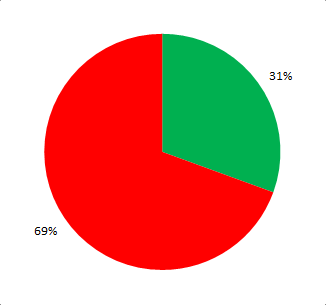
\includegraphics[width=1.5cm, height=1.5cm]{diag.png}
\end{minipage}
\\[0.5cm]

\begin{minipage}{0.5\textwidth}
Б4. ``Как часто за последний учебный год Вы давали открытые уроки (занятия, мероприятия)?''
\end{minipage}
& 3 & 5 & 
\begin{minipage}{1.55cm}
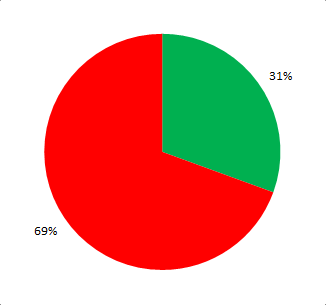
\includegraphics[width=1.5cm, height=1.5cm]{diag.png}
\end{minipage}
\\[0.5cm]

\begin{minipage}{0.5\textwidth}
Б21. ``Как часто коллеги-педагоги (преподаватели, воспитатели) за последний учебный год посещали Ваши занятия и мероприятия (не открытые, т.е. которые вы специально не готовили)?''
\end{minipage}
& 7 & 2 &
\begin{minipage}{1.55cm}
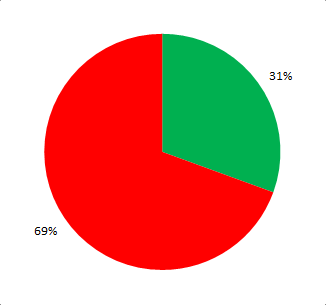
\includegraphics[width=1.5cm, height=1.5cm]{diag.png}
\end{minipage}
\\[0.5cm]

\begin{minipage}{0.5\textwidth}
Б22. ``Как часто за последний учебный год Вам приходилось бывать на занятиях и мероприятиях (не открытых, т.е. которые они специально не готовили) педагогов (преподавателей, воспитателей) Вашей образовательной организации?''
\end{minipage}
& 3 & 5 &
\begin{minipage}{1.55cm}
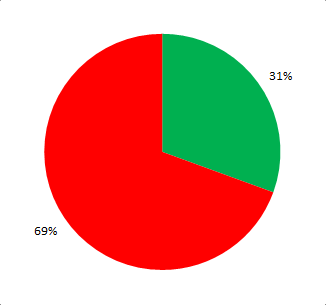
\includegraphics[width=1.5cm, height=1.5cm]{diag.png}
\end{minipage}
\\
\end{tabular}


\end{frame}



%=====================================================
\begin{frame}{2.2.5. Тип организации взаимодействия по обмену опытом}


\tiny

На диаграмме представлен результат по вопросу Б24.
\bigskip

\begin{itemize}
\item [Б24] После посещения занятий  и мероприятий (открытых и неоткрытых)  в нашей образовательной организации  обычно:
\end{itemize}

\begin{columns}
\begin{column}{0.4\textwidth} 
\centering
\includegraphics[width=4cm, height=4cm]{pie225.png}
\end{column}
\begin{column}{0.6\textwidth} \begin{tabular}{l} 
 Занятие (мероприятие) обсуждается \\
один на один с преподавателем --- \valBBEansA\ (\valBBEansAp\%)  \\[0.5cm] 
Занятие (мероприятие)   анализируется \\
с администрацией ---   \valBBEansB\ (\valBBEansBp\%) \\[0.5cm]
Организуется групповое обсуждение \\
занятия (мероприятия) всеми \\
присутствовавшими на нем  --- \valBBEansC\ (\valBBEansCp\%) \\[0.5cm]
Ничего не происходит ---  \valBBEansD\ (\valBBEansDp\%) \\[0.5cm]
\end{tabular}
\end{column}
\end{columns}

\end{frame}




%=====================================================
\begin{frame}{3. Уровень вертикального доверия}

Вступление с определением понятия области исследования и отсылкой к подробностям в Методических рекомендациях.

\end{frame}




%=====================================================
\begin{frame}{3.1.1. Декларируемый уровень доверия к руководству (сводный результат) }

\tiny

На диаграмме представлен сводный результат по вопросу Б18:
\bigskip


Б18. Согласие с тем, что руководство образовательной организации защищает интересы респоднента и заботится о нем: ``Согласны ли Вы с тем, что руководство образовательной организации защищает Ваши интересы и заботится о Вас?''
\bigskip

\begin{columns}
\begin{column}{0.4\textwidth} 
\centering
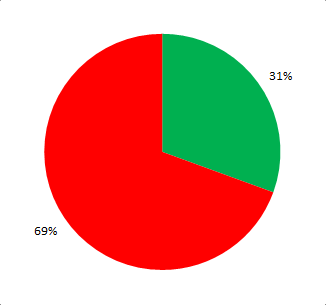
\includegraphics[width=4cm, height=4cm]{diag.png}
\end{column}
\begin{column}{0.6\textwidth} \begin{tabular}{l} 
 Ответили утвердительно   \\ 
(``да'' или ``скорее да, чем нет'')  ---   \numExpC\ (33\%) \\ [0.3cm]
 Ответили отрицательно  \\ 
 (``нет'' или ``скорее нет, чем да'') ---  \numExpD\ (67\%) \\ 
\end{tabular}
\end{column}
\end{columns}

\end{frame}



%=====================================================
\begin{frame}{3.1.2. Декларируемый уровень доверия к руководству (группы по возрасту) }

\tiny

На диаграмме представлен результат по вопросу Б18 с разбивкой по возрасту:
\bigskip

\centering 

\begin{tabular}{|l|c|c|c|c|} \hline
& до 25 лет &  25 -- 35  лет &  36 -- 55 лет & свыше 55 лет \\ \hline
Ответили утвердительно & & & & \\
(``да'' или ``скорее да, чем нет'')  & \valCAByesNumA     &   \valCAByesNumB         &   \valCAByesNumC  & \valCAByesNumD \\ \hline
Ответили отрицательно  & & & & \\
(``нет'' или ``скорее нет, чем да'') & \valCABnoNumA  &  \valCABnoNumB    &   \valCABnoNumC   & \valCABnoNumD  \\ \hline
\end{tabular}
\bigskip

\begin{tabular}{cccc}
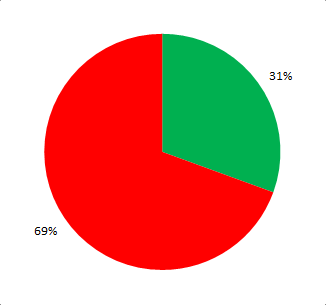
\includegraphics[width=2.2cm, height=2.2cm]{diag.png} & 
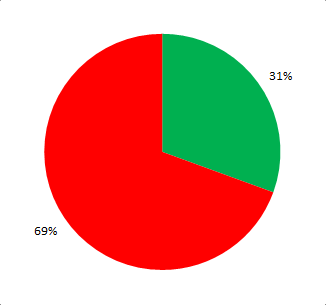
\includegraphics[width=2.2cm, height=2.2cm]{diag.png} & 
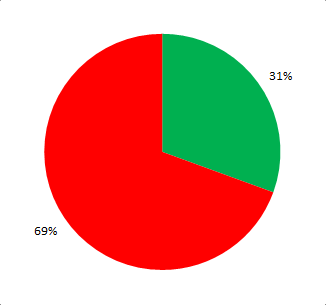
\includegraphics[width=2.2cm, height=2.2cm]{diag.png} & 
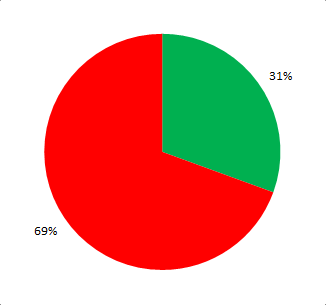
\includegraphics[width=2.2cm, height=2.2cm]{diag.png} \\
до 25 лет &  25 -- 35  лет &  36 -- 55 лет & свыше 55 лет \\
\end{tabular}

\end{frame}



%=====================================================
\begin{frame}{3.1.3. Декларируемый уровень доверия к руководству \\ (группы по квалификационной категории) }

\tiny

На диаграммах представлен результат по вопросу Б18 с разбивкой по квалификационной категории:
\bigskip

\centering 

\begin{tabular}{|l|c|c|c|c|c|} \hline
  & Не проходил &  Аттестован & 2-я &  1-я  & Высшая \\ 
 &  аттестацию   &  на соотв. & категория &  категория  & категория \\ \hline
Ответили  & & & & & \\
утвердительно  & \valCACyesNumA &  \valCACyesNumB  &  \valCACyesNumC  & \valCACyesNumD  & \valCACyesNumE \\ 
(Да, cкорее да...) & & & & & \\ \hline
Ответили   & & & & & \\
отрицательно & \valCACnoNumA  & \valCACnoNumB & \valCACnoNumC  & 
\valCACnoNumD & \valCACnoNumE \\ 
(Нет, cкорее нет...) & & & & & \\ \hline
\end{tabular}

\bigskip

\begin{tabular}{ccccc}
\includegraphics[width=2cm, height=2cm]{pie313a.png} & 
\includegraphics[width=2cm, height=2cm]{pie313b.png} & 
\includegraphics[width=2cm, height=2cm]{pie313c.png} & 
\includegraphics[width=2cm, height=2cm]{pie313d.png} & 
\includegraphics[width=2cm, height=2cm]{pie313e.png} \\
 Не проходили &  Аттестованы & 2-я &  1-я  & Высшая \\ 
  аттестацию   &  на соотв. & категория &  категория  & категория \\ 
\end{tabular}

\end{frame}




%=====================================================
\begin{frame}{3.2. Фактический уровень вертикального доверия}

\tiny

В данном разделе анализируются ответы на вопросы Б15, Б16, Б17:
\bigskip

\begin{itemize}

\item [Б15] Личное обращение к руководителю ОУ по своей инициативе по вопросам преподавания и воспитания конкретных обучающихся. ``Как часто Вы лично за последний учебный год по своей инициативе обращались (обсуждали, советовались) по вопросам преподавания и воспитания конкретных обучающихся (воспитанников) или классов (групп) к директору (заведующему)?'

\item [Б16] Личное обращение к администрации (замам руководителя) по своей инициативе по вопросам преподавания и воспитания конкретных обучающихся. ``Как часто Вы лично за последний учебный год по своей инициативе обращались (обсуждали, советовались) по вопросам преподавания и воспитания конкретных обучающихся (воспитанников) или классов (групп) к зам. директора (заведующего)?'

\item [Б17] Личное обращение к заведующим кафедрами  по своей инициативе по вопросам преподавания и воспитания конкретных обучающихся. ``Как часто Вы лично за последний учебный год по своей инициативе обращались (советовались, обсуждали) по вопросам преподавания и воспитания конкретных обучающихся (воспитанников) или классов (групп)  к заведующим кафедрами  (методобъединений, отделений)?''

\end{itemize}

\end{frame}



%=====================================================
\begin{frame}{3.2.1. Частотность обращения педагогов к администрации по вопросам преподавания и воспитания (сводный результат) }


\tiny

На диаграмме представлен сводный результат по вопросам Б15, Б16, Б17.
\bigskip

\begin{columns}
\begin{column}{0.4\textwidth} 
\centering
\includegraphics[width=4cm, height=4cm]{pie321.png}
\end{column}
\begin{column}{0.6\textwidth} \begin{tabular}{l} 
 Ответили утвердительно   \\ 
(``Несколько раз в неделю'' или ``Раз в неделю'')  ---   \valCBAyesNum\ (\valCBAyesNumP\%) \\ [0.3cm]
 Ответили отрицательно  \\ 
 (``Раз в месяц'' или ``Еще реже'') ---  \valCBAnoNum\ (\valCBAnoNumP\%) \\ 
\end{tabular}
\end{column}
\end{columns}

\end{frame}



%=====================================================
\begin{frame}{3.2.2. Частотность обращения педагогов к администрации по вопросам преподавания и воспитания (группы по возрасту) }

\tiny

На диаграмме представлен результат по вопросам Б15, Б16, Б17 с разбивкой по возрасту.
\bigskip

\centering 

\begin{tabular}{|l|c|c|c|c|} \hline
& до 25 лет &  25 -- 35  лет &  36 -- 55 лет & свыше 55 лет \\ \hline
Ответили утвердительно & & & & \\
(``да'' или ``скорее да, чем нет'')  & \valCBByesNumA  & \valCBByesNumB   &   \valCBByesNumC    & \valCBByesNumD  \\ \hline
Ответили отрицательно  & & & & \\
(``нет'' или ``скорее нет, чем да'') & \valCBBnoNumA     &  \valCBBnoNumB  &   \valCBBnoNumC     & \valCBBnoNumD  \\ \hline
\end{tabular}
\bigskip

\begin{tabular}{cccc}
\includegraphics[width=2.2cm, height=2.2cm]{pie322a.png} & 
\includegraphics[width=2.2cm, height=2.2cm]{pie322b.png} & 
\includegraphics[width=2.2cm, height=2.2cm]{pie322c.png} & 
\includegraphics[width=2.2cm, height=2.2cm]{pie322d.png} \\
до 25 лет &  25 -- 35  лет &  36 -- 55 лет & свыше 55 лет \\
\end{tabular}

\end{frame}



%=====================================================
\begin{frame}{3.2.3. Частотность обращения педагогов к администрации по вопросам преподавания и воспитания (группы по квалификационной категории) }

\tiny

На диаграммах представлен результат по вопросам Б15, Б16, Б17 с разбивкой по квалификационной категории.
\bigskip

\centering 

\begin{tabular}{|l|c|c|c|c|c|} \hline
  & Не проходил &  Аттестован & 2-я &  1-я  & Высшая \\ 
 &  аттестацию   &  на соотв. & категория &  категория  & категория \\ \hline
Ответили  & & & & & \\
утвердительно  & \valCBCyesNumA  & \valCBCyesNumB  & \valCBCyesNumC & 
\valCBCyesNumD  & \valCBCyesNumE  \\ 
(Раз в месяц или чаще) & & & & & \\ \hline
Ответили   & & & & & \\
отрицательно & \valCBCnoNumA & \valCBCnoNumB  &  \valCBCnoNumC  & 
\valCBCnoNumD & \valCBCnoNumE \\ 
(Раз в полугодие или реже) & & & & & \\ \hline
\end{tabular}

\bigskip

\begin{tabular}{ccccc}
\includegraphics[width=2cm, height=2cm]{pie323a.png} & 
\includegraphics[width=2cm, height=2cm]{pie323b.png} & 
\includegraphics[width=2cm, height=2cm]{pie323c.png} & 
\includegraphics[width=2cm, height=2cm]{pie323d.png} & 
\includegraphics[width=2cm, height=2cm]{pie323e.png} \\
 Не проходили &  Аттестованы & 2-я &  1-я  & Высшая \\ 
  аттестацию   &  на соотв. & категория &  категория  & категория \\ 
\end{tabular}

\end{frame}



%=====================================================
\begin{frame}{3.2.4. Данные по вопросам, включенным в блок ``Фактический уровень вертикального доверия'' }

\tiny

\begin{tabular}{lccl}

 & Раз в месяц  & Один раз в  &\\
 & или чаще    & полугодие  &\\
 &      &  или реже &\\

\begin{minipage}{0.5\textwidth}
Б15.  Как часто Вы лично за последний учебный год по своей инициативе обращались (обсуждали, советовались) по вопросам преподавания и воспитания конкретных обучающихся (воспитанников) или классов (групп) к директору (заведующему)?
\end{minipage}
& \valCBDyesNumA & \valCBDnoNumA &
\begin{minipage}{1.55cm}
\includegraphics[width=1.5cm, height=1.5cm]{pie324a.png}
\end{minipage}
\\[0.7cm]

\begin{minipage}{0.5\textwidth}
Б16. Как часто Вы лично за последний учебный год по своей инициативе обращались (обсуждали, советовались) по вопросам преподавания и воспитания конкретных обучающихся (воспитанников) или классов (групп) к зам. директора (заведующего)?
\end{minipage}
& \valCBDyesNumB & \valCBDnoNumB &
\begin{minipage}{1.55cm}
\includegraphics[width=1.5cm, height=1.5cm]{pie324b.png}
\end{minipage}
\\[0.7cm]

\begin{minipage}{0.5\textwidth}
Б17. Как часто Вы лично за последний учебный год по своей инициативе обращались (советовались, обсуждали) по вопросам преподавания и воспитания конкретных обучающихся (воспитанников) или классов (групп)  к заведующим кафедрами  (методобъединений, отделений)?
\end{minipage}
& \valCBDyesNumC & \valCBDnoNumC &
\begin{minipage}{1.55cm}
\includegraphics[width=1.5cm, height=1.5cm]{pie324c.png}
\end{minipage}
\\

\end{tabular}


\end{frame}




%=====================================================
\begin{frame}{4.1. Позиция администрации по отношению горизонтального контроля}


\tiny

На диаграмме представлен результат по вопросу Б11:
\bigskip

\begin{itemize}
\item [Б11] Действия сотрудников при возникновении конфликтной ситуации (по мнению руководства). ``Если у педагогов (преподавателей, воспитателей) возникла конфликтная ситуация (например, по разделению обязанностей), какие пути ее урегулирования они должны использовать прежде всего?''
\end{itemize}

\begin{columns}
\begin{column}{0.4\textwidth} 
\centering
\includegraphics[width=4cm, height=4cm]{pie41.png}
\end{column}
\begin{column}{0.6\textwidth} \begin{tabular}{l} 
 Обратиться к руководству --- \valDAansA\ (\valDAansAp\%)  \\[0.5cm] 
Решить конфликтный вопрос самостоятельно,  \\
договорившись между собой ---   \valDAansB\ (\valDAansBp\%) \\[0.5cm]
Обсудить ситуацию с другими коллегами --- \valDAansC\ (\valDAansCp\%) \\[0.5cm]
Другое --- \valDAansD\ (\valDAansDp\%) \\[0.5cm]
\end{tabular}
\end{column}
\end{columns}

\end{frame}



%=====================================================
\begin{frame}{4.2. Позиция педагогических работников по отношению горизонтального контроля}

\tiny

В данном разделе анализируются ответы на вопросы Б12, Б20, Б29:
\bigskip

\begin{itemize}

\item [Б12] Действия сотрудников при возникновении конфликтной ситуации (по мнению сотрудников). ``Если у Вас возникла конфликтная ситуация с коллегой (например, по разделению обязанностей), как Вы ее решаете чаще всего?''

\item [Б20] Варианты реакции на несправедливость по отношению к обучающемуся, проявленную педагогом. ``Если Вам покажется, что коллега-педагог (преподаватель, воспитатель) проявил несправедливость по отношению к обучающемуся (воспитаннику), что Вы сделаете?''

\item [Б29] Готовность выразить свое отношение к опоздавшему(ей) на свое занятие коллеге. ``Выразите ли Вы свое отношение к коллеге, который/ая опоздал/а на проводимое им/ей занятие или мероприятие?''

\end{itemize}

\end{frame}



%=====================================================
\begin{frame}{4.2.а. Позиция педагогических работников по отношению горизонтального контроля}


\tiny

На диаграмме представлен результат по вопросу Б12:
\bigskip

\begin{itemize}
\item [Б12] Действия сотрудников при возникновении конфликтной ситуации (по мнению сотрудников). ``Если у Вас возникла конфликтная ситуация с коллегой (например, по разделению обязанностей), как Вы ее решаете чаще всего?''
\end{itemize}

\begin{columns}
\begin{column}{0.4\textwidth} 
\centering
\includegraphics[width=4cm, height=4cm]{pie42_a_.png}
\end{column}
\begin{column}{0.6\textwidth} \begin{tabular}{l} 
Обращаетесь к руководству --- \valDBAansA\ (\valDBAansAp\%)  \\[0.5cm] 
Договариваетесь с коллегой ---  \valDBAansB\ (\valDBAansBp\%) \\[0.5cm]
Обсуждаете с другими коллегами --- \valDBAansC\ (\valDBAansCp\%) \\[0.5cm]
Другое --- \valDBAansD\ (\valDBAansDp\%) \\[0.5cm]
\end{tabular}
\end{column}
\end{columns}

\end{frame}



%=====================================================
\begin{frame}{4.2.б. Позиция педагогических работников по отношению горизонтального контроля}


\tiny

На диаграмме представлен результат по вопросу Б20:
\bigskip

\begin{itemize}
\item [Б20] Варианты реакции на несправедливость по отношению к обучающемуся, проявленную педагогом. ``Если Вам покажется, что коллега-педагог (преподаватель, воспитатель) проявил несправедливость по отношению к обучающемуся (воспитаннику), что Вы сделаете?''
\end{itemize}

\begin{columns}
\begin{column}{0.4\textwidth} 
\centering
\includegraphics[width=4cm, height=4cm]{pie42_b_.png}
\end{column}
\begin{column}{0.6\textwidth} \begin{tabular}{l} 
Утешите обучающегося (воспитанника) --- \valDBBansA\ (\valDBBansAp\%)  \\[0.5cm] 
Обсудите ситуацию с этим коллегой ---   \valDBBansB\ (\valDBBansBp\%) \\[0.5cm]
Обратитесь к администрации --- \valDBBansC\ (\valDBBansCp\%) \\[0.5cm]
Ничего, вдруг это мне просто показалось --- \valDBBansD\ (\valDBBansDp\%) \\[0.5cm]
Другое --- \valDBBansE\ (\valDBBansEp\%) \\[0.5cm]
\end{tabular}
\end{column}
\end{columns}

\end{frame}



%=====================================================
\begin{frame}{4.2.в. Позиция педагогических работников по отношению горизонтального контроля}


\tiny

На диаграмме представлен результат по вопросу Б29:
\bigskip

\begin{itemize}
\item [Б29] Готовность выразить свое отношение к опоздавшему(ей) на свое занятие коллеге. ``Выразите ли Вы свое отношение к коллеге, который/ая опоздал/а на проводимое им/ей занятие или мероприятие?''
\end{itemize}

\begin{columns}
\begin{column}{0.4\textwidth} 
\centering
\includegraphics[width=4cm, height=4cm]{pie42_c_.png}
\end{column}
\begin{column}{0.6\textwidth} \begin{tabular}{l} 
 Ответили утвердительно   \\ 
(``да'' или ``скорее да, чем нет'')  ---   \valDBCyesNum\ (\valDBCyesNumP\%) \\ [0.3cm]
 Ответили отрицательно  \\ 
 (``нет'' или ``скорее нет, чем да'') ---  \valDBCnoNum\ (\valDBCnoNumP\%) \\ 
\end{tabular}
\end{column}
\end{columns}

\end{frame}




%=====================================================
\begin{frame}{5.1. Удовлетворенность работой (сводный результат) }


\tiny

На диаграмме представлен сводный результат по вопросам Б31, Б32.
\bigskip

\begin{columns}
\begin{column}{0.4\textwidth} 
\centering
\includegraphics[width=4cm, height=4cm]{pie71.png}
\end{column}
\begin{column}{0.6\textwidth} \begin{tabular}{l} 
 Ответили утвердительно   \\ 
(``да'' или ``скорее да, чем нет'')  ---   \valGAyesNumP\% \\ [0.3cm]
 Ответили отрицательно  \\ 
 (``нет'' или ``скорее нет, чем да'') ---  \valGAnoNumP\% \\ 
\end{tabular}
\end{column}
\end{columns}

На диаграмме представлены сводные результаты ответов на вопросы этого блока. Важными аспектами оценки в данном случае является: 
\begin {itemize}
\item Устраивает ли Вас уровень удовлетворенности работой сотрудников, если нет, что можно предпринять (если это необходимо) для его повышения?

\item Что в Вашей образовательной организации в наибольшей степени  влияет на уровень удовлетворенности работой?

\item Насколько высокий уровень удовлетворенности повышает эффективность деятельности организации?
\end {itemize}


\end{frame}



%=====================================================
\begin{frame}{5.2. Удовлетворенность работой (по группам) }

\tiny

На диаграмме представлен результат по вопросам Б31, Б32 с разбивкой по возрасту.

\begin{tabular}{cccc}
\includegraphics[width=2.2cm, height=2.2cm]{pie72a.png} & 
\includegraphics[width=2.2cm, height=2.2cm]{pie72b.png} & 
\includegraphics[width=2.2cm, height=2.2cm]{pie72c.png} & 
\includegraphics[width=2.2cm, height=2.2cm]{pie72d.png} \\
до 25 лет &  25 -- 35  лет &  36 -- 55 лет & свыше 55 лет \\
\end{tabular}
\bigskip

То же с разбивкой по квалификационной категории.

\begin{tabular}{ccccc}
\includegraphics[width=2cm, height=2cm]{pie73a.png} & 
\includegraphics[width=2cm, height=2cm]{pie73b.png} & 
\includegraphics[width=2cm, height=2cm]{pie73c.png} & 
\includegraphics[width=2cm, height=2cm]{pie73d.png} & 
\includegraphics[width=2cm, height=2cm]{pie73e.png} \\
 Не проходили &  Аттестованы & 2-я &  1-я  & Высшая \\ 
  аттестацию   &  на соотв. & категория &  категория  & категория \\ 
\end{tabular}
\bigskip

На диаграмме - данные ответов на вопросы об удовлетворенности разных возрастных и категориальных групп. Однороден ли коллектив в своих позициях относительно удовлетворенности работой? Должен ли быть разным уровень удовлетворенности различных групп сотрудников? 
\end{frame}



%=====================================================
\begin{frame}{5.3. Удовлетворенность работой (группы по квалификационной категории) }

\tiny

На диаграммах представлен результат по вопросам Б31, Б32 с разбивкой по квалификационной категории.
\bigskip

\centering 

\begin{tabular}{|l|c|c|c|c|c|} \hline
  & Не проходил &  Аттестован & 2-я &  1-я  & Высшая \\ 
 &  аттестацию   &  на соотв. & категория &  категория  & категория \\ \hline
Ответили  & & & & & \\
утвердительно  & \valGCyesNumA  &  \valGCyesNumB  & \valGCyesNumC  & \valGCyesNumD  & \valGCyesNumE \\ 
(Да, cкорее да...) & & & & & \\ \hline
Ответили   & & & & & \\
отрицательно & \valGCnoNumA   & \valGCnoNumB  & \valGCnoNumC  & 
\valGCnoNumD & \valGCnoNumE \\ 
(Нет, cкорее нет...) & & & & & \\ \hline
\end{tabular}

\bigskip

\begin{tabular}{ccccc}
\includegraphics[width=2cm, height=2cm]{pie73a.png} & 
\includegraphics[width=2cm, height=2cm]{pie73b.png} & 
\includegraphics[width=2cm, height=2cm]{pie73c.png} & 
\includegraphics[width=2cm, height=2cm]{pie73d.png} & 
\includegraphics[width=2cm, height=2cm]{pie73e.png} \\
 Не проходили &  Аттестованы & 2-я &  1-я  & Высшая \\ 
  аттестацию   &  на соотв. & категория &  категория  & категория \\ 
\end{tabular}

\end{frame}




%=====================================================
\begin{frame}{6.1.1 Актуальные профессиональные связи}

\begin{columns} 
\begin{column}{0.75\textwidth} 
\centering
          \includegraphics[width=8cm, height=8cm]{graph5_1a.png}
\end{column}
\begin{column}{0.25\textwidth} 

\tiny
Граф \textcolor{blue}{всех} профессиональных связей построен по ответам на два вопроса:
\smallskip

1. ``Если у Вас возникают профессиональные проблемы, то с кем из коллег Вы советуетесь, к кому обращаетесь за помощью?''
\smallskip

2. ``Назовите тех коллег, к кому по разным причинам (помощь, знакомство с чужим опытом и пр.) Вы чаще ходите на занятия в настоящее время?''
\smallskip

Отображены \textcolor{blue}{все} связи. 
\smallskip

Размер узла пропорционален количеству входящих стрелок.

\end{column}
\end{columns}
\end{frame}



%=====================================================
\begin{frame}{6.1.2. Актуальные профессиональные связи (взаимные)}

\begin{columns}
\begin{column}{0.75\textwidth} 
\centering
          \includegraphics[width=8cm, height=8cm]{graph6_1b.png}
\end{column}
\begin{column}{0.25\textwidth} 

\tiny
Граф \textcolor{blue}{взаимных} профессиональных связей также построен по ответам на два вопроса:
\smallskip

- ``Если у Вас возникают профессиональные проблемы, то с кем из коллег Вы советуетесь, к кому обращаетесь за помощью?''
\smallskip

- ``Назовите тех коллег, к кому по разным причинам (помощь, знакомство с чужим опытом и пр.) Вы чаще ходите на занятия в настоящее время?''
\smallskip

На диаграмме отображены только \textcolor{blue}{взаимные} связи.
\smallskip

Размер узла пропорционален количеству связей.
\smallskip

Изолированные узлы не показаны.
\end{column}
\end{columns}
\end{frame}



%=====================================================
\begin{frame}{Раздел 6.2.1. Потенциальные профессиональные связи}

\begin{columns}
\begin{column}{0.75\textwidth} 
\centering
          \includegraphics[width=8cm, height=8cm]{graph5_2a.png}
\end{column}
\begin{column}{0.25\textwidth} 

\tiny
Граф \textcolor{blue}{всех потенциальных} профессиональных связей построен по ответам на два вопроса:
\smallskip

1. ``Кого из коллег Вы хотели бы видеть в составе вновь организованной группы для решения какой-либо проблемы в области преподавания и воспитания?''
\smallskip

2. ``Как вы считаете, кого из коллег Вам было бы полезно видеть на своих уроках, занятиях и мероприятиях?''
\smallskip

Отображены \textcolor{blue}{все} связи. 
\smallskip

Размер узла пропорционален количеству входящих стрелок.

\end{column}
\end{columns}
\end{frame}



%=====================================================
\begin{frame}{Раздел 6.2.2. Потенциальные профессиональные связи (взаимные)}

\begin{columns} 
\begin{column}{0.75\textwidth}
\centering
          \includegraphics[width=8cm, height=8cm]{graph6_2b.png}
\end{column}
\begin{column}{0.25\textwidth} 

\tiny
Граф \textcolor{blue}{потенциальных взаимных} профессиональных связей также построен по ответам на два вопроса:
\smallskip

- ``Кого из коллег Вы хотели бы видеть в составе вновь организованной группы для решения какой-либо проблемы в области преподавания и воспитания?''
\smallskip

- ``Кого из коллег Вам было бы полезно видеть на своих уроках, занятиях и мероприятиях?''
\smallskip

На диаграмме отображены только \textcolor{blue}{взаимные} потенциальные профессиональные связи.
\smallskip

Размер узла пропорционален количеству связей.
\smallskip

Изолированные узлы не показаны.

\end{column}
\end{columns}
\end{frame}



%=====================================================
\begin{frame}{Раздел 6.3. Профессиональное лидерство}


\tiny
Рейтинг построен по ответам на четыре вопроса:
\smallskip

- ``С кем из коллег Вы советуетесь, к кому обращаетесь за помощью?''
\smallskip

- ``К кому Вы чаще ходите на занятия?''
\smallskip

- ``Кого из коллег Вы хотели бы видеть в составе группы для решения проблем в области преподавания и воспитания?''
\smallskip

- ``Кого из коллег Вам было бы полезно видеть на своих уроках?''
\smallskip

\end{frame}




%=====================================================
\begin{frame}{7. Уровень сложности личных связей }

Текст. Вступление с определением понятия области исследования и отсылкой к подробностям в Методических рекомендациях

\end{frame}



%=====================================================
\begin{frame}{7.1. Удовлетворенность работой (сводный результат) }


\tiny

На диаграмме представлен сводный результат по вопросам Б31, Б32:
\bigskip

\begin{columns}
\begin{column}{0.4\textwidth} 
\centering
\includegraphics[width=4cm, height=4cm]{pie71.png}
\end{column}
\begin{column}{0.6\textwidth} \begin{tabular}{l} 
 Ответили утвердительно   \\ 
(``да'' или ``скорее да, чем нет'')  ---   \valGAyesNum\ (\valGAyesNumP\%) \\ [0.3cm]
 Ответили отрицательно  \\ 
 (``нет'' или ``скорее нет, чем да'') ---  \valGAnoNum\ (\valGAnoNumP\%) \\ 
\end{tabular}
\end{column}
\end{columns}

\end{frame}



%=====================================================
\begin{frame}{7.2. Удовлетворенность работой (группы по возрасту) }

\tiny

На диаграмме представлен результат по вопросам Б31, Б32 с разбивкой по возрасту:
\bigskip

\centering 

\begin{tabular}{|l|c|c|c|c|} \hline
& до 25 лет &  25 -- 35  лет &  36 -- 55 лет & свыше 55 лет \\ \hline
Ответили утвердительно & & & & \\
(``да'' или ``скорее да, чем нет'')  & \valGByesNumA     & \valGByesNumB    &   \valGByesNumC    & \valGByesNumD  \\ \hline
Ответили отрицательно  & & & & \\
(``нет'' или ``скорее нет, чем да'') & \valGBnoNumA     &  \valGBnoNumB    &   \valGBnoNumC     & \valGBnoNumD  \\ \hline
\end{tabular}
\bigskip

\begin{tabular}{cccc}
\includegraphics[width=2.2cm, height=2.2cm]{pie72a.png} & 
\includegraphics[width=2.2cm, height=2.2cm]{pie72b.png} & 
\includegraphics[width=2.2cm, height=2.2cm]{pie72c.png} & 
\includegraphics[width=2.2cm, height=2.2cm]{pie72d.png} \\
до 25 лет &  25 -- 35  лет &  36 -- 55 лет & свыше 55 лет \\
\end{tabular}

\end{frame}



%=====================================================
\begin{frame}{7.3. Удовлетворенность работой (группы по квалификационной категории) }

\tiny

На диаграммах представлен результат по вопросам Б31, Б32 с разбивкой по квалификационной категории:
\bigskip

\centering 

\begin{tabular}{|l|c|c|c|c|c|} \hline
  & Не проходил &  Аттестован & 2-я &  1-я  & Высшая \\ 
 &  аттестацию   &  на соотв. & категория &  категория  & категория \\ \hline
Ответили  & & & & & \\
утвердительно  & \valGCyesNumA  &  \valGCyesNumB  & \valGCyesNumC  & \valGCyesNumD  & \valGCyesNumE \\ 
(Да, cкорее да...) & & & & & \\ \hline
Ответили   & & & & & \\
отрицательно & \valGCnoNumA   & \valGCnoNumB  & \valGCnoNumC  & 
\valGCnoNumD & \valGCnoNumE \\ 
(Нет, cкорее нет...) & & & & & \\ \hline
\end{tabular}

\bigskip

\begin{tabular}{ccccc}
\includegraphics[width=2cm, height=2cm]{pie73a.png} & 
\includegraphics[width=2cm, height=2cm]{pie73b.png} & 
\includegraphics[width=2cm, height=2cm]{pie73c.png} & 
\includegraphics[width=2cm, height=2cm]{pie73d.png} & 
\includegraphics[width=2cm, height=2cm]{pie73e.png} \\
 Не проходили &  Аттестованы & 2-я &  1-я  & Высшая \\ 
  аттестацию   &  на соотв. & категория &  категория  & категория \\ 
\end{tabular}

\end{frame}



%=====================================================
\begin{frame}{7.4. Данные по вопросам, включенным в блок ``Удовлетворенность работой'' }

\tiny


\begin{tabular}{lccl}

 & Да & Нет &\\

\begin{minipage}{0.62\textwidth}
Б31. ``Вы считаете, что полностью реализуете свой потенциал на работе?''
\end{minipage}
& \valGDyesNumA & \valGDnoNumA &
\begin{minipage}{1.55cm}
\includegraphics[width=1.5cm, height=1.5cm]{pie74a.png}
\end{minipage}
\\[0.5cm]

\begin{minipage}{0.62\textwidth}
Б32.  ``Вы считаете, что Вас ценят в коллективе по достоинству?''
\end{minipage}
& \valGDyesNumB & \valGDnoNumB &
\begin{minipage}{1.55cm}
\includegraphics[width=1.5cm, height=1.5cm]{pie74b.png}
\end{minipage}
\end{tabular}

\end{frame}




%=====================================================
\begin{frame}{8. Заключение}

\tiny 
Вы получили первичные данные по проведенному исследованию. Эти результаты мы предоставляем только Вам и именно Вы должны решить, что и в каком объеме стоит обсуждать с коллегами. 
\smallskip

Следует принимать во внимание, что, как и всякое исследование, основанное на опросе, это отнюдь не претендует на то, чтобы поставить окончательный диагноз. Объективность полученных данных сильно зависит от условий, в которых они были получены (насколько тревожны были отвечающие, как они были проинструктированы и т.д.) Но если кто-то и осведомлен об этом, то это именно Вы.  Вы лучше всех знаете, можно ли этим данным доверять.
\smallskip

Но  если данные покажутся Вам значимыми, то они могут быть основанием для принятия решений, основанных не только на интуиции, но и на данных. Надеемся, что это исследование принесет пользу Вам и организации.


\end{frame}

%-----------------------------------------------------
\begin{frame}{}

\tiny 
Отчёт разрабатывали и готовили:

\begin{itemize}

\item Ушаков Константин Михайлович, д.п.н., профессор Института образования НИУ Высшая школа экономики, главный редактор журнала "Директор школы".

\item Фишбейн Дмитрий Ефимович, к.п.н., доцент Института образования НИУ Высшая школа экономики, главный редактор "Журнала руководителя управления образованием".

\item Яворский Ростислав Эдуардович, к.п.н., доцент Департамента анализа данных и искусственного интеллекта НИУ Высшая школа экономики.

\item Шиварев Павел Васильевич, заместитель главного редактора "Журнала руководителя управления образованием".

\item Кухарев Антон Иванович, магистр образования, заместитель директора МБОО СОШ № 25 г. Альметьевска Республики Татарстан

\end{itemize}

\end{frame}



%=====================================================
\begin{frame}{8.1. Актуальные профессиональные связи }

\tiny

В данном разделе анализируются ответы на вопросы С6, С8:
\bigskip

\begin{itemize}

\item [С6] Если у Вас возникают профессиональные проблемы, то с кем из коллег Вы советуетесь, к кому обращаетесь за помощью?

\item [С8] Назовите тех коллег, к кому по разным причинам (помощь, знакомство с чужим опытом и пр.) Вы чаще ходите на занятия в настоящее время?

\end{itemize}

\end{frame}



%=====================================================
\begin{frame}{Раздел 7.2.1. Граф ``Потенциальные профессиональные связи в организации''}

\begin{columns}
\begin{column}{0.75\textwidth} 
\centering
          \includegraphics[width=8cm, height=8cm]{graph8_2a.png}
\end{column}
\begin{column}{0.25\textwidth} 

\tiny
Граф построен по ответам на вопросы С4, С7.
\smallskip

Отображены все связи. 
\smallskip

Размер узла пропорционален количеству связей.
\smallskip

Жёлтым цветом обозначен руководитель организации.
\bigskip

Всего связей --- \valHBAlinks.

\end{column}
\end{columns}
\end{frame}



%=====================================================
\begin{frame}{8.2.2. Значимость взаимопосещений (группы по возрасту) }

\tiny

На диаграмме представлен результат по вопросу Б22 с разбивкой по возрасту:
\bigskip

\centering 

\begin{tabular}{|l|c|c|c|c|} \hline
& до 25 лет &  25 -- 35  лет &  36 -- 55 лет & свыше 55 лет \\ \hline
Ответили утвердительно & & & & \\
(``Раз в неделю'' или ``Раз в месяц'')  & \valHBByesNumA     &   \valHBByesNumB         &  \valHBByesNumC        & \valHBByesNumD \\ \hline
Ответили отрицательно  & & & & \\
(``Раз в полугодие'' или ``Ещё реже'') & \valHBBnoNumA     &   \valHBBnoNumB         &   \valHBBnoNumC        & \valHBBnoNumD  \\ \hline
\end{tabular}
\bigskip

\begin{tabular}{cccc}
\includegraphics[width=2.2cm, height=2.2cm]{pie822a.png} & 
\includegraphics[width=2.2cm, height=2.2cm]{pie822b.png} & 
\includegraphics[width=2.2cm, height=2.2cm]{pie822c.png} & 
\includegraphics[width=2.2cm, height=2.2cm]{pie822d.png} \\
до 25 лет &  25 -- 35  лет &  36 -- 55 лет & свыше 55 лет \\
\end{tabular}

\end{frame}



%=====================================================
\begin{frame}{8.2.3. Значимость взаимопосещений (группы по квалификационной категории) }

\tiny

На диаграммах представлен результат по вопросу Б22 с разбивкой по квалификационной категории:
\bigskip

\centering 

\begin{tabular}{|l|c|c|c|c|c|} \hline
  & Не проходил &  Аттестован & 2-я &  1-я  & Высшая \\ 
 &  аттестацию   &  на соотв. & категория &  категория  & категория \\ \hline
Ответили  & & & & & \\
утвердительно  & \valHBCyesNumA   &  \valHBCyesNumB &  \valHBCyesNumC  & \valHBCyesNumD  & \valHBCyesNumE \\ 
(Раз в месяц или чаще) & & & & & \\ \hline
Ответили   & & & & & \\
отрицательно & \valHBCnoNumA  & \valHBCnoNumB & \valHBCnoNumC  & 
\valHBCnoNumD & \valHBCnoNumE \\ 
(Раз в полугодие или реже) & & & & & \\ \hline
\end{tabular}

\bigskip

\begin{tabular}{ccccc}
\includegraphics[width=2cm, height=2cm]{pie823a.png} & 
\includegraphics[width=2cm, height=2cm]{pie823b.png} & 
\includegraphics[width=2cm, height=2cm]{pie823c.png} & 
\includegraphics[width=2cm, height=2cm]{pie823d.png} & 
\includegraphics[width=2cm, height=2cm]{pie823e.png} \\
 Не проходили &  Аттестованы & 2-я &  1-я  & Высшая \\ 
  аттестацию   &  на соотв. & категория &  категория  & категория \\ 
\end{tabular}

\end{frame}



%=====================================================
\begin{frame}{Раздел 7.3. Профессиональное лидерство}

\tiny
Под профессиональным лидерством мы понимаем то, в какой мере данный сотрудник значим (следовательно и выбираем) для других членов коллектива в контекстах напрямую связанных с работой.
\bigskip

В данном разделе анализируются ответы на вопросы С1, С4, С6, С7, С8.
\bigskip

\begin{itemize}

\item [С1] Кто из коллег, по вашему мнению, являются лучшими педагогами (преподавателями, воспитателями) вашей образовательной организации?

\item [С4] Кого из коллег Вы хотели бы видеть в составе вновь организованной группы для решения какой-либо проблемы в области преподавания и воспитания?

\item [С6] Если у Вас возникают профессиональные проблемы, то с кем из коллег Вы советуетесь, к кому обращаетесь за помощью?

\item [С7] Как вы считаете, кого из коллег Вам было бы полезно видеть на своих уроках, занятиях и мероприятиях?

\item [С8] Назовите тех коллег, к кому по разным причинам (помощь, знакомство с чужим опытом и пр.) Вы чаще ходите на занятия в настоящее время?

\end{itemize}

\end{frame}



%=====================================================
\begin{frame}{8.4. Принятый формат анализа посещений}


\tiny

На диаграмме представлен результат по вопросу Б24:
\bigskip

\begin{itemize}
\item [Б24] Обычные действия после посещения открытых и неподготовленных занятий. ``После посещения занятий  и мероприятий (открытых и неоткрытых)  в нашей образовательной организации  обычно''
\end{itemize}

\begin{columns}
\begin{column}{0.4\textwidth} 
\centering
\includegraphics[width=4cm, height=4cm]{pie84.png}
\end{column}
\begin{column}{0.6\textwidth} \begin{tabular}{l} 
Занятие (мероприятие) обсуждается один\\
 на один с преподавателем --- \valHDansA\ (\valHDansAp\%)  \\[0.5cm] 
Занятие (мероприятие)   анализируется\\
 с администрацией ---  \valHDansB\ (\valHDansBp\%) \\[0.5cm]
Организуется групповое обсуждение\\ 
занятия (мероприятия) всеми \\
присутствовавшими на нем --- \valHDansC\ (\valHDansCp\%) \\[0.5cm]
Ничего не происходит --- \valHDansD\ (\valHDansDp\%) \\[0.5cm]
\end{tabular}
\end{column}
\end{columns}

\end{frame}




\end{document}


